\section{RePlay System}
This section describes RePlay's user interface, context detection, and system architecture.
%RePlay is a desktop application that allows users to search for contextually-relevant video clips for any accessibility-enabled desktop application. It leverages large online video corpora, searching video caption text for relevant moments. The RePlay prototype investigates the efficacy and challenges of cross-app contextual search.

\begin{figure}[b!]
\centering
\vspace{-0.2in}
  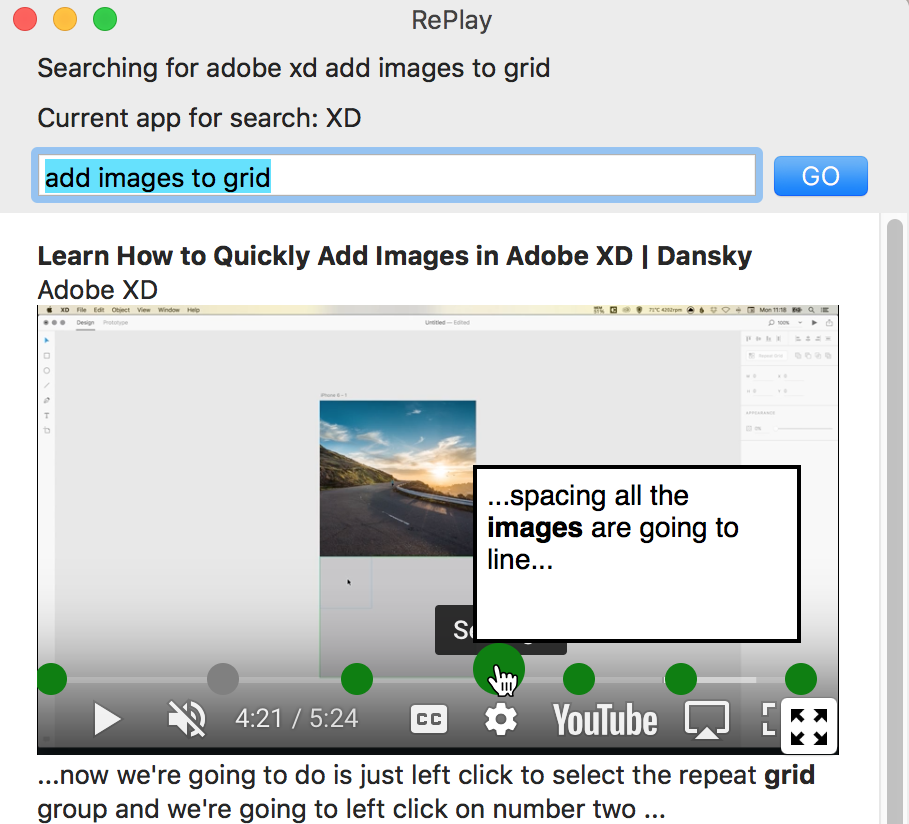
\includegraphics[width=\textwidth]{replay/figures/green_markers.png}
  \caption{RePlay overlays green markers on the video timeline to indicate moments where the captions match a user's search term. Mousing over a marker shows a pop-up with an excerpt from the captions at that moment; clicking it plays the video from that moment. }~\label{fig:replay-green_markers}
%   \Description[A screenshot showing green markers overlaid on a video result in RePlay.]{A screenshot showing green markers overlaid on a video result in RePlay. The user has searched for ``add images to grid'' in Adobe XD, and the top video result is titled ``Learn how to quickly add images in Adobe XD''. The video timeline has green dots on it, and the mouse is hovering over one. A pop-up shows a caption excerpt that says: ``...spacing all the images are going to line...'' with the word ``images'' bolded.}
  \vspace{-0.2in}
\end{figure}

\subsection{User interface}
The RePlay panel (\autoref{fig:replay-interface}) can be positioned and sized as desired; its default size is 465px \texttimes 1055px. It is designed to fit next to the user's primary applications to minimize switching windows. The narrow pane makes videos small but easier to browse and watch in context. The interface comprises a status area, search field, and video results.

The status area updates as the user works, displaying the name of the last tool clicked and the current application (\autoref{fig:replay-status}). ``Tools'' refer to interface elements or commands within an application. The status area provides awareness of what context RePlay will use for search (\textit{i.e.,} so the user does not need to include the application name in their search query). When the user initiates a search, the status area updates to show the query (\autoref{fig:replay-interface}b).

As the user works, the search field updates with the name of the last tool clicked (\autoref{fig:replay-status}). Users can edit or delete it to form their own query. Pressing the \textsc{go} button or return key triggers a search. RePlay displays the top five resulting videos, each cued to start at a relevant moment. A two-line excerpt from that moment's caption appears below the video with query words highlighted in bold \cite{Hearst2009}.

Often, videos have multiple moments that may be relevant. RePlay renders green markers on the video timeline to indicate these moments. Mousing over a marker invokes a pop-up text area displaying a caption excerpt with words from the query in bold (\autoref{fig:replay-green_markers}). This pop-up obscures YouTube's default thumbnail pop-up but provides more useful information, as software videos tend to show an entire screen and shrinking this to a thumbnail makes it hard to see. Clicking a marker starts the video from that moment. 

\begin{figure}[b!]
\centering
\vspace{-0.2in}
  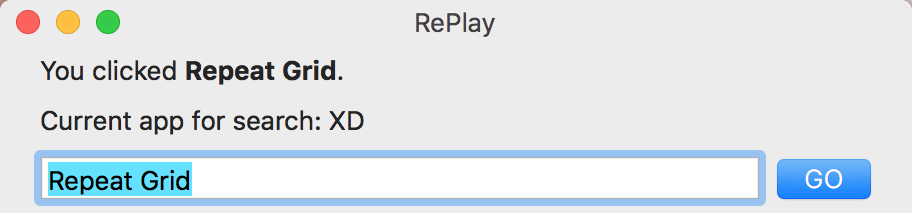
\includegraphics[width=\textwidth]{replay/figures/replay_status.png}
  \caption{RePlay's status area displays tool names after they are clicked and adds them to the search field. }~\label{fig:replay-status}
%   \Description[A screenshot of RePlay's status area.]{A screenshot of RePlay's status area. It reads, ``you clicked Repeat Grid'', and has the tool name ``Repeat Grid'' included in the search field.}
  \vspace{-0.2in}
\end{figure}


RePlay also displays contextual cues \cite{Ekstrand2011} on search results (\autoref{fig:replay-context_cues}). For each video, RePlay lists the three most-recently used applications that are mentioned in the video (\autoref{fig:replay-context_cues}a). This list is especially useful when users move between applications and want videos that mention both the current and recent applications. RePlay renders grey timeline markers to indicate moments where recently used tools are mentioned (\autoref{fig:replay-context_cues}b). Caption pop-ups italicize tool names.


\begin{figure}[b!]
\centering
\vspace{-0.2in}
  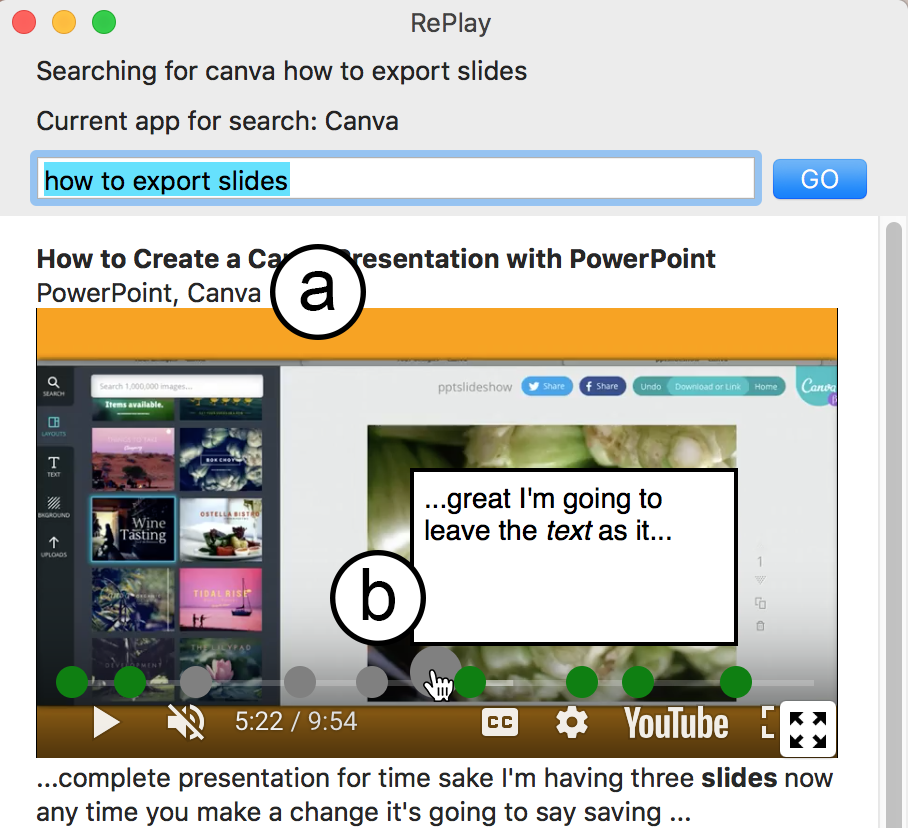
\includegraphics[width=\textwidth]{replay/figures/context_cues.png}
  \caption{RePlay displays contextual cues based on recent app and tool use. a) RePlay lists the three most recent apps that the video mentions. b) Grey markers indicate mentions of recently-used tools. In this example, the user recently used the ``text'' tool in Canva. Mousing over a marker shows a caption excerpt; clicking a marker plays the video. }~\label{fig:replay-context_cues}
%   \Description[A screenshot showing grey markers overlaid on a video result in RePlay.]{A screenshot showing grey markers overlaid on a video result in RePlay. The user has searched for ``how to export slides'' in Canva, and the top video result is titled ``How to create a canva presentation with PowerPoint''. The video timeline has grey dots on it, and the mouse is hovering over one. A pop-up shows a caption excerpt that says: ``...great I'm going to leave the text as it...'' with the word ``text'' italicized.}
  \vspace{-0.2in}
\end{figure}

RePlay's panel shows all results at the same time, allowing users to quickly skim multiple videos, and browse other results while one video plays. This ability to ``see inside'' multiple resources from a single page increases foraging efficiency \cite{Vermette2017, Glassman2016, Pavel2013}. 

Clicking the full-screen button in a video's bottom-right corner opens the video in a separate window that stays above all other windows while it is open, so that users can watch a video at a larger size when desired.

When the user switches to a new application and clicks a tool, RePlay automatically searches for the application name. This seeds the panel with app-relevant videos that give users a starting point.

\subsection{Detecting application context}
RePlay uses contextual information to augment a user's query and search within video results. The motivation for context-augmented search is to increase relevance, especially when users don't know what to ask for. However, if not done well, adding terms has the opposite effect: excluding relevant results and/or presenting irrelevant ones \cite{Finkelstein2002}. We tried several heuristics with RePlay; the current implementation includes the three most recent applications and tools.

\subsubsection{How to detect context?}
RePlay leverages \textsc{os} accessibility \textsc{api}s to detect every click. On each click event, RePlay retrieves the name of the click's source application, the type of element clicked, and the element's accessibility description (when present). If the element is a button, checkbox, text field, slider, or menu item, RePlay stores it as a recent tool and updates the status area and search field with the tool's name. If the user switched applications since their last click, RePlay updates its status area to reflect the new application, and resets its list of recent tools.

\subsubsection{Challenges with detecting context via accessibility}
Extracting accessibility text obviates the need for hard-coded knowledge about specific applications. The challenge of this system-wide approach is that despite platform accessibility guidelines, applications vary widely in what accessibility they offer and how \cite{Hurst2010}.

In Mac\-OS, RePlay can always extract the application name and menu items. Buttons and other interface elements have accessibility labels in many applications (\textit{e.g.,} Adobe \textsc{xd}, Microsoft Office, iMovie, Tableau, Sketch), but not in others (often long-existing software, \textit{e.g.,} Photoshop). Applications differ in which accessibility fields they support and what information is in what field. For example, tool names may be in the \textit{Title}, \textit{Help}, \textit{Description}, or \textit{Value} attribute. RePlay checks all four, preferring them in that order. RePlay also gathers accessibility information for websites, as long as browser accessibility access is enabled. It is by default in Safari, and as an option in Chrome. Many sites implement accessibility labels (\textit{e.g., } Canva, Wordpress, Sketchpad, Snappa, G Suite). Those that do not still include some information by default (\textit{e.g.}, text area contents via the \textit{Value} attribute). RePlay infers website names from the \textsc{url} and website title.

\subsection{Video search \& ranking}
RePlay leverages existing online video search engines to retrieve video results. It then finds and ranks relevant clips within these videos (\autoref{fig:replay-system}). RePlay's architecture requires no prior understanding of the applications or videos; it relies on captions for clip extraction and ranking. Video authors often talk about things they are doing and provide tips about tools; captions thus provide narrative information beyond the visual content in the video that can be useful for learners.

\begin{figure}[b!]
\centering
\vspace{-0.2in}
  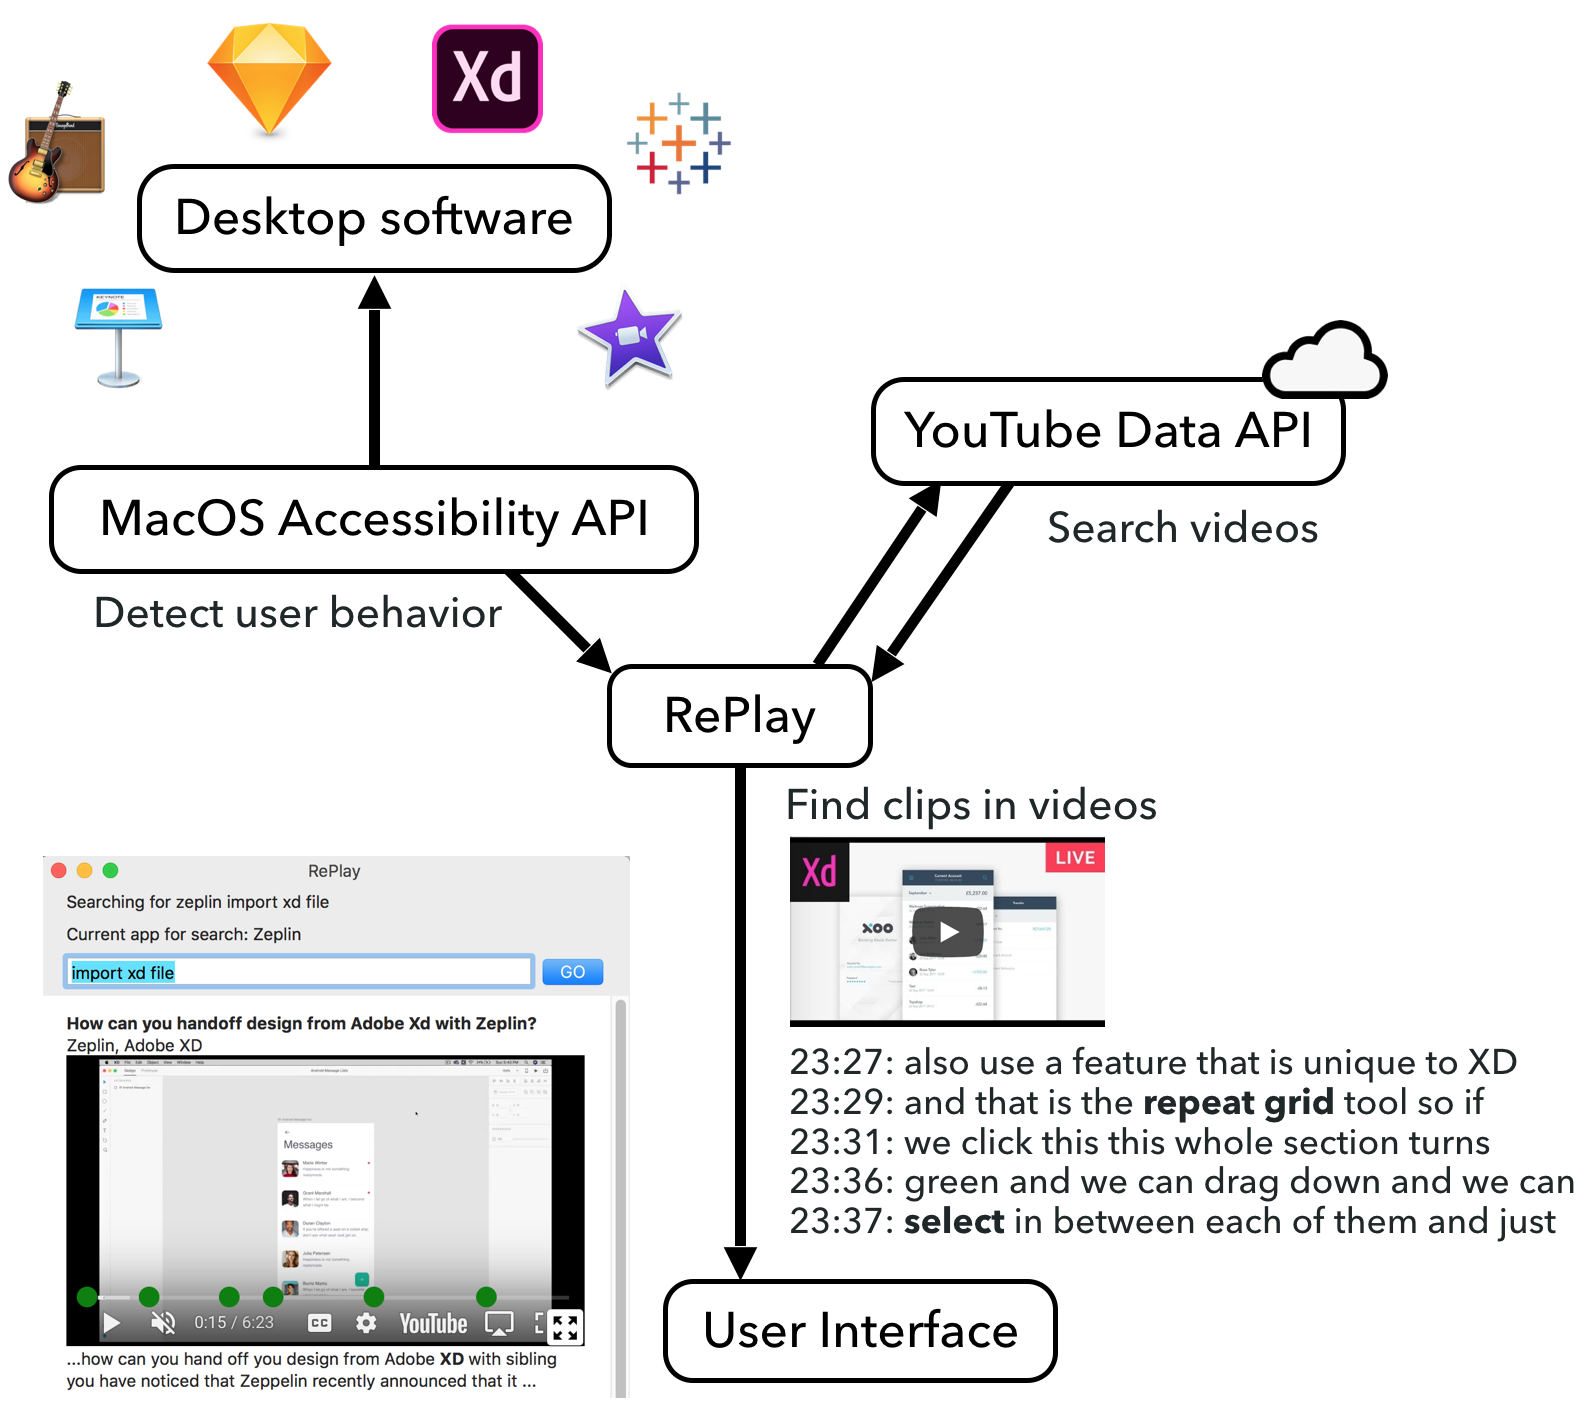
\includegraphics[width=\textwidth]{replay/figures/replay-system.png}
  \caption{RePlay uses accessibility \textsc{api}s to detect user context, which it uses to augment the user's query and to search and rank videos. RePlay finds matching clips by searching video captions for the user's query and recent tool names. }~\label{fig:replay-system}
%   \Description[A diagram showing the different components of RePlay and how they communicate.]{A diagram showing the different components of RePlay and how they communicate. The MacOS Accessibility API detects user behavior from desktop software and sends this to RePlay. RePlay searches videos using the YouTube Data API. RePlay finds clips in these videos and displays them in the user interface.}
  \vspace{-0.2in}
\end{figure}

\subsubsection{Available data}
RePlay's current video corpus comprises all English videos on YouTube that have a caption track. Most do: YouTube auto-generates captions by default. We used YouTube for its popularity and captions; any video search engine with an \textsc{api} could be used. For example, Vimeo (\url{vimeo.com}) and Dailymotion (\url{dailymotion.com}) also provide \textsc{api} access to videos and captions.

\subsubsection{Searching}
Video search requires more steps than document search, because captions are obtained separately. This two-step search means that issuing multiple queries with context terms added (such as tool usage) like prior work \cite{Ekstrand2011} would be too slow. To speed responses, RePlay constructs and issues a single query concatenating the current application's name with the user's query. Leaving context terms out of the query also ensures that the user-provided search terms are not ``washed out''. RePlay queries YouTube and selects its top five video results that have English captions and mention the current application in any of the title, description, or captions (to avoid results that may contain other keywords but do not pertain to the current application).

\subsubsection{Finding clips and re-ranking videos}
Several techniques automatically extract instructional video clips from screencasts of software use. The dominant approach leverages application usage \cite{Grossman2010, Lafreniere2014, Chi2012, Wang2018}, requiring that the video be recorded in an instrumented version of the software. Alternatively, computer vision can detect tool-selection events \cite{Pongnumkul2011, Matejka2011}, even without prior knowledge about the specific software \cite{Banovic2012}. To be application-independent and embed online videos directly without waiting to download and process them, RePlay instead uses metadata and caption text to rank and segment videos. 

For each video result, RePlay divides its captions into 30-second segments, searching each for the queried keywords (with stop words removed) and names of the three most-recently used tools in the current application. It ranks all segments by the total number of keyword matches. To break ties it uses number of tool name matches. The highest-ranked segment determines the video's start time. Timeline markers denote the top ten segments: green for those with a query term; grey if only a tool is mentioned. RePlay re-orders the video results based on the total number of matching clips. To break ties it uses the total number of matching keywords within the clips.

Although automatic captions are far from perfect, we found them to be sufficient for searching in RePlay. Captions are already an approximation of what the demonstrator is doing, so despite some errors, they work well enough for identifying potentially relevant moments. Having any aids for navigating within videos is still an improvement over standard viewers. Still, future systems could allow viewers to easily correct errors as they watch to improve caption accuracy for future viewers.

\subsection{Implementation}
RePlay is implemented as a Mac\-OS application in Swift. It uses the Mac\-OS Accessibility \textsc{api} to extract information from input events. For both studies, RePlay used a whitelist to only detect clicks in certain applications and websites. A blacklist could be used instead; we explore this in the discussion.

When a search is triggered, RePlay queries the YouTube Data \textsc{api}'s \texttt{search} method, which returns an ordered list of video \textsc{id}s. For each \textsc{id}, RePlay checks if English captions are available using YouTube's \texttt{get\_video\_info} method. If they are, this method's response includes a \textsc{url} that RePlay follows to obtain subtitles in \textsc{xml}, with time stamps for every 5 to 10 words. A search that returns all new videos can take up to a few minutes to finish depending on network speed, due to the multiple requests needed to retrieve captions for each video. To speed up future searches, RePlay caches all retrieved captions locally (since they are pure text, this takes up little space). This could be further improved by proactively caching results for common search queries and buffering results as they come in. RePlay's video player is implemented in Javascript on a custom server; it embeds a YouTube video in an \texttt{iframe}, cues it to the given start time, and overlays timeline markers and pop-up captions. RePlay displays each video by loading this web player in a Swift \texttt{WKWebView} object. 